% BRED


One of the central cellular processes underlying development is transcriptional regulation. During development, changes in transcription factor activity induce chromatin modifications, chromatin remodeling and ultimately a differential recruitment of the basal transcriptional machinery [66]. Modeling the dynamics of gene regulation is therefore essential to better understand why a cellular dynamic processes progresses through several steps, and what goes wrong in the case of disease.

The dynamics of gene regulation has classically been studied using time series data [23]. When dynamic processes progress asynchronously, such as in hematopoiesis, time series data are usually obtained by sorting different transition states and assessing bulk gene expression and transcription factor binding within the population [67–70]. Alternatively, time series data can also be generated by synchronizing the dynamic process between cells. However, issues with time-resolution, heterogeneity and good in vivo synchronization models can often limit the predictive power of the dynamic models of gene regulation which can be constructed [23]. Combining single-cell snapshot data with trajectory inference can now in principle construct an accurate time-series dataset for every cell population both in vivo and in vitro, while avoiding issues with heterogeneity. Initially, several pioneering studies demonstrated the potential of this approach in single cells using single-cell qPCR data for selected sets of 10 to 50 transcription factors [71–75]. With the advent of genome wide single-cell technologies, the models of dynamic gene regulation can now be made even more complete while avoiding a prior bias to well studied transcription factors [17,30,76,77] and several methods have already been developed specifically tuned towards single-cell data [78–80].

The power of a dynamic network approach in single cells is not only that it allows the identification of transcription factors specifically regulating a specific state, but also how these factors then induce sets of genes necessary for regulating the next wave of transcription changes (Figure 1B). Such a gene regulatory cascade was described during cellular reprogramming from mouse embryonic fibroblasts to induced pluripotent stem cells, where SOX2 was shown to activate a series of other transcription factors which, together with SOX2, induces pluripotency [72]. Transition states are frequently associated with particular subnetworks of transcriptional regulators, as was shown in a direct reprogramming setting from fibroblasts to neurons [77]. Several studies have highlighted how some regulatory links can be very dynamic while others show evidence of being static during consecutive developmental stages [74,75]. Regulatory network motifs can also be extracted from the regulatory network [74], some of which can have interesting properties in dynamic systems [81,82]. In branching trajectories dynamic regulatory networks can also be used to study the regulators important for a particular branch [17,75,79] (Figure 1C).


\begin{figure}[htb!]
	\centering
	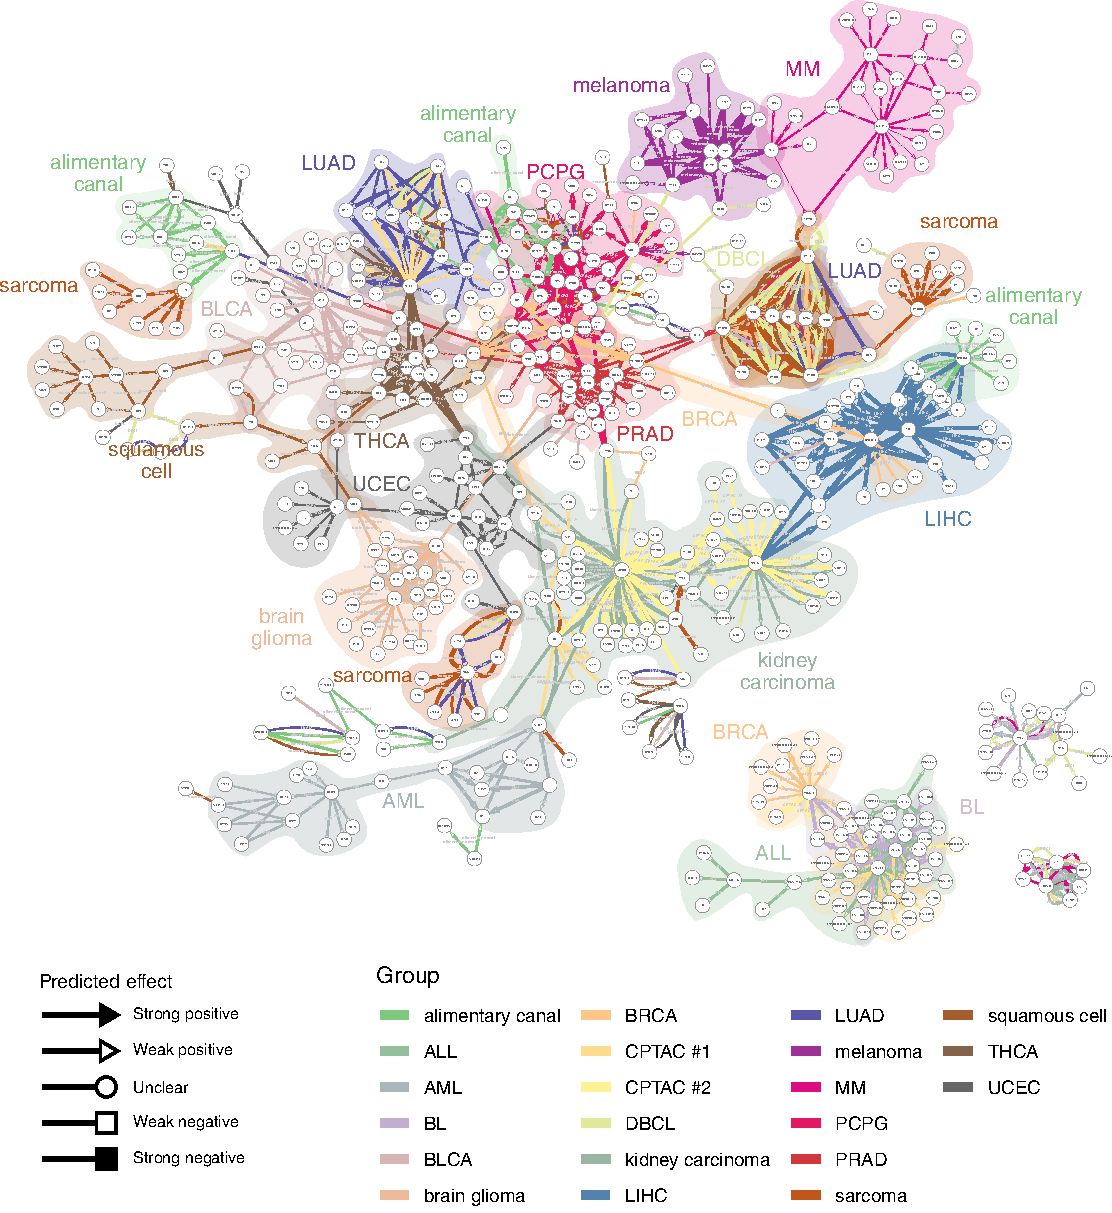
\includegraphics[width=\linewidth]{fig/tcga/grouped_interactions.pdf} 
	\caption{
		A
	}
	\label{fig:tcga}
\end{figure}



\clearpage
\section{References}
\printbibliography[heading=none]
